\section{Overall System}

\todo

\begin{figureBox}[label={fig:System layout}, width=1.0\linewidth]{System layout}
    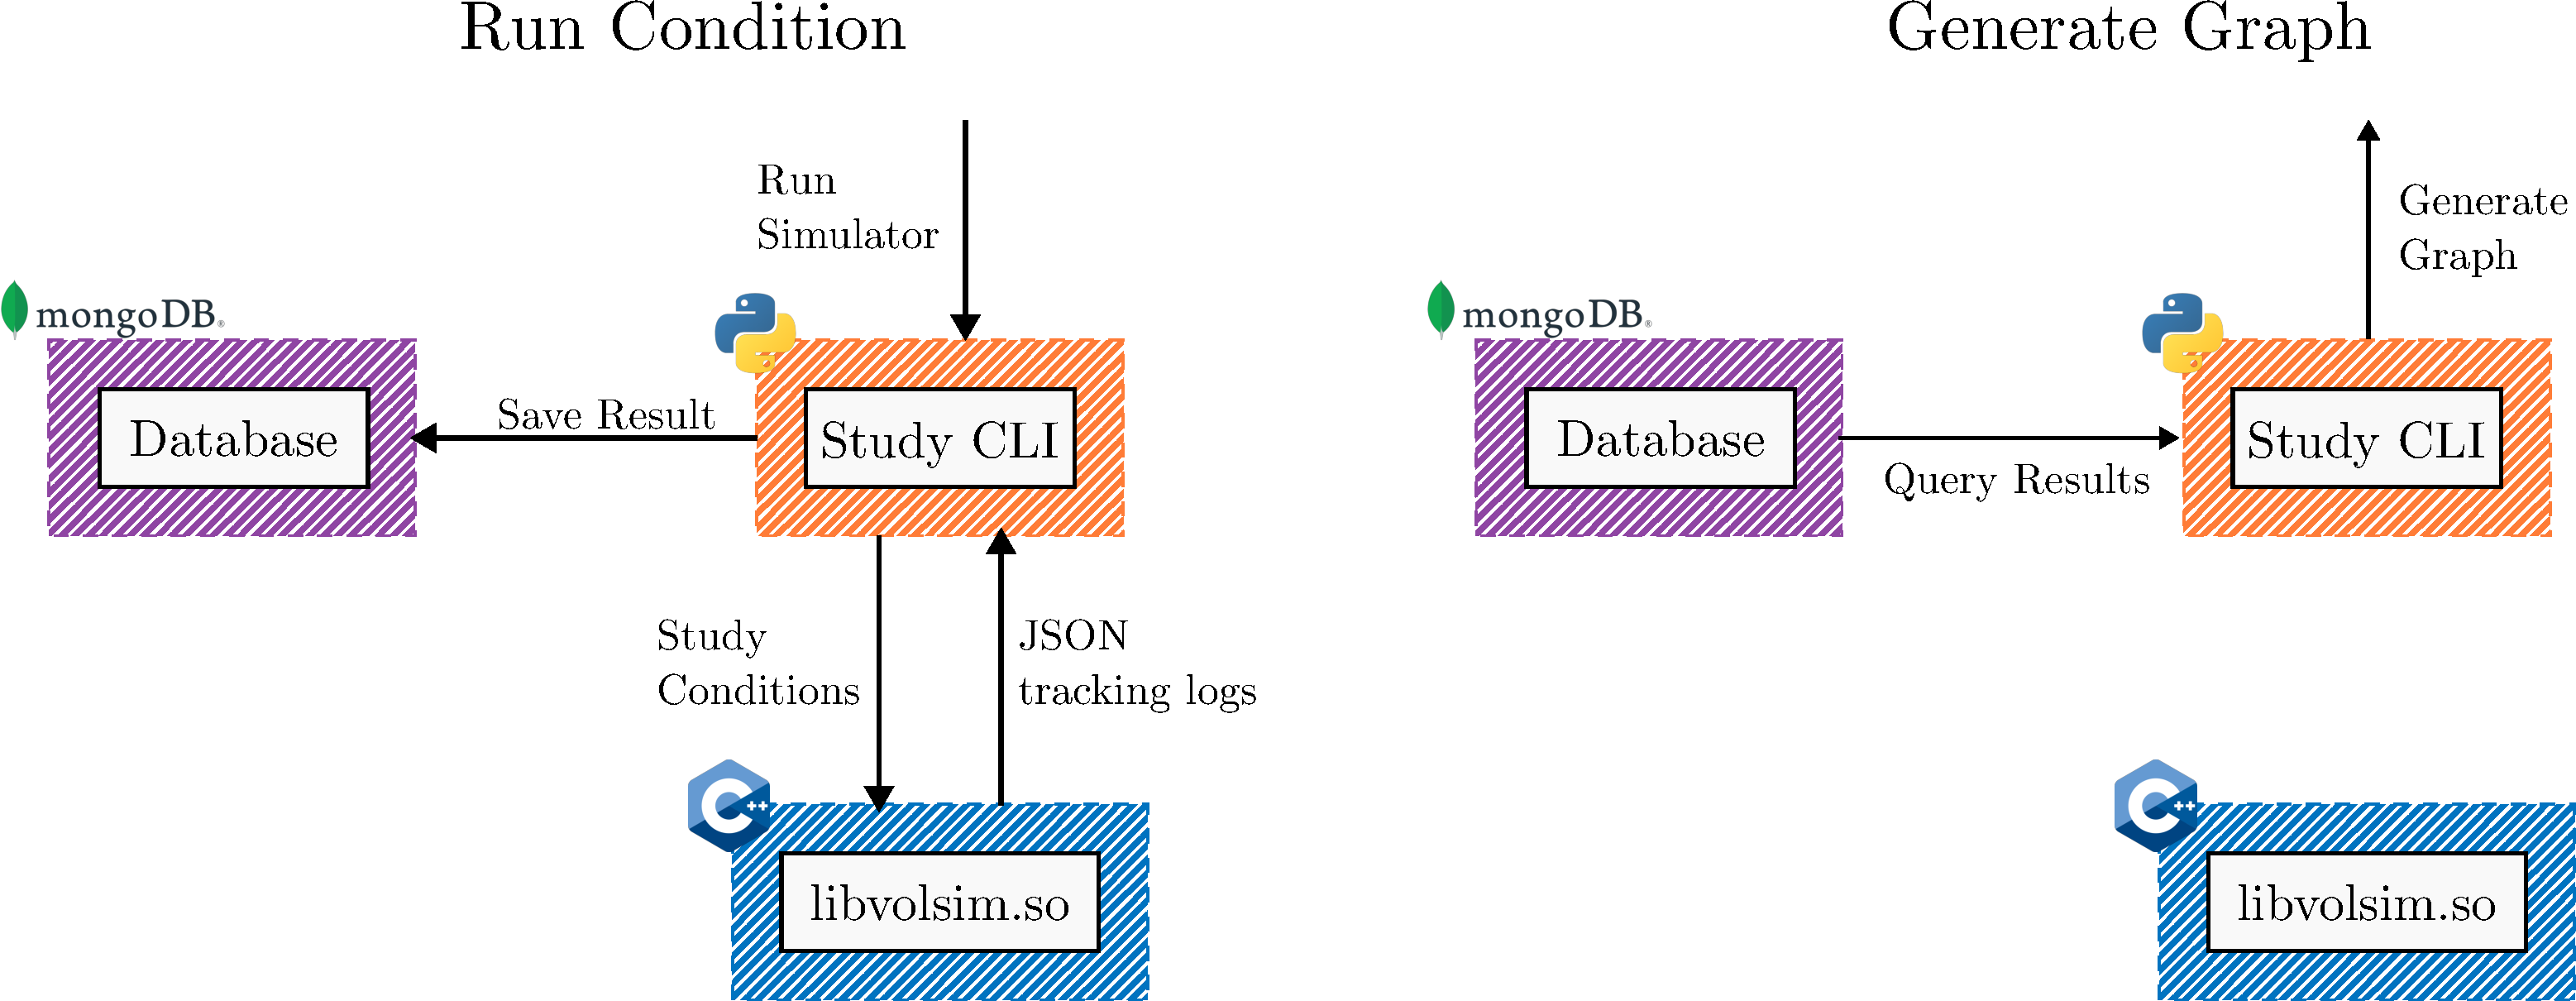
\includegraphics[width = 1.0\linewidth]{./implementation/figures/overall-system.pdf}
\end{figureBox}

\subsection{Build System}

The build system plays a crucial role in compiling the simulator and rendering system, as well as running the user study. This complex system requires the compilation of C++, CUDA, and Python code, and the management of large ML models and object files for rendering, as well as managing things like camera drivers. Portability is essential to ensure the user study can be conducted on various systems. Given our previous experiences, the build system often presents a significant bottleneck in the development process. To address these challenges, we have chosen nix for its declarative nature and ease of dependency management, including the capability to modify packages globally using overlays.

\subsubsection{Overview}
\begin{enumerate}
	\item Draw a diagram of the build system (simplified)
	\item The build system is split into two parts the simulator, and the user study.
	\item Show how the simulator is compiled as a shared library and called from the user study.
\end{enumerate}

The build system provides two main functionalities compiling the simulator (written in c++) as a shared library, and providing development environments for running the user study (written in python). This functionality is all available through a $\texttt{nix flake}$ interface as can be seen in List~\ref{list:main-nix-flake}. 

\codeBoxFile[label = {list:main-nix-flake}]{shell}{./implementation/code/flake-show.sh}{Terminal}

\subsubsection{libvolsim.so}

You can build our simulator as a shared library using the following simple command in List~\ref{list:nix-build}:
\codeBoxFile[label = {list:nix-build}]{shell}{./implementation/code/nix-build.sh}{Terminal}

Although this might look like a simple command, it is doing a lot of work behind the scenes. Firstly it will go and fetch all the dependencies required to build the simulator, from source (or a public binary cache). You do not need to have any of the dependencies installed on your system, as nix will manage all of this for you. 

Our packages configures:
\begin{enumerate}
	\item \textbf{CUDA:} As we use CUDA in our simulator, we need to build the CUDA toolkit. Luckily nix allows you to build it in a more fine grained way, so you can build just pick and choose the parts you need. We use CUDA Deep Neural Network library (cuDNN), CUDA Basic Linear Algebra Subprograms library (cuBLAS),CUDA Random Number Generation library (cuRAND), CUDA Dense Linear Solver library (cuSOLVER) along with the required libaries to interact with them. We override and recompile OpenCV and Dlib to be CUDA enabled. \tocite
	\item \textbf{MKL:} We use the Intel Math Kernel Library (MKL) for some of our linear algebra operations as it significantly faster than the default BLAS library. We override and recompile OpenCV and DLIB to use the MKL BLAS libaries. \tocite
	\item \textbf{Azure Kinect Sensor SDK:} We use our own nix package for the Azure Kinect SDK, as it was not packaged. This package provides the required drivers and stubs for the Azure Kinect camera to run. \tocite
	\item \textbf{OpenGL:} We download and configure \texttt{GLFW} (Light weight OpenGL utility library) and \texttt{GLAD} (Hardware specific OpenGL drivers) for OpenGL. \tocite
	\item \textbf{Tracking models:} We download and configure Dlib and MediaPipe machine learning libraries that we use for our tracking models. We also automatically download the required two required models for DLIB (\texttt{shape\_predictor\_5\_face\_landmarks},\texttt{mmod\_human\_face\_detector}) from the internet (verified by hash). We also download and build OpenCV for managing our images. \tocite
\end{enumerate}

Once all the dependencies are built, the simulator is compiled written into the nix store as package with a shared library \texttt{libvolsim.so} and all the files the simulator depends on (tracking models, obj files, shaders). This shared library can be called from the user study to run the simulator. An overview of the final package contains can be seen in List~\ref{list:libvolsim}.

\codeBoxFile[label = {list:libvolsim}]{shell}{./implementation/code/libvolsim.sh}{Terminal}

\subsubsection{Dev Environments}

To run our user study, we have created a development environment that contains all the dependencies required to run the user study and sets up an alias that allows you to run the study via a CLI easily as can be seen in List~\ref{list:study}. 

\codeBoxFile[label = {list:study}]{shell}{./implementation/code/study.sh}{Terminal}

As we also use out CLI to analyse the results of the user study, we have also created a development environment that contains all the dependencies required to run the analysis and completely reproduce the graphs and tables in this documents. \\

We also created a development shell to automatically launch and manage a local mongodb database for storing the results of the user study. This included gui tools for viewing the database editing the database (mongodb-compass). This can be activated by running the command you can see in List~\ref{list:mongo}.

\codeBoxFile[label = {list:mongo}]{shell}{./implementation/code/mongo.sh}{Terminal}

\subsection{Extra work}

One of the major downsides of using nix is that if something is not already packaged by another user you have to package it yourself. Luckily almost everything we needed was already packaged in nixpkgs, but we did have to package a few things ourselves. Usually if something is not packaged in nixpkgs, it is because it is not a widely used package, or it is a pain to package. 

\subsubsection{Azure Kinect Package}

The first thing we had to package was the Azure Kinect SDK. This was not packaged in nixpkgs, and the only official package was a (not very well made) out of date Ubuntu package. To get it working in nix we have to manually patch the rpaths (run-time search path hard-coded in an executable file) in the file and fix some build and driver issues.  Microsoft officially stopped supporting the Azure Kinect in August 2023 (\tocite) so we decided to package a fork of \texttt{https://github.com/microsoft/Azure-Kinect-Sensor-SDK} that fixed a lot of the issues we had. All in all this was quite difficult and took about a week. We haven't upstreamed this to nixpkgs yet but might do in the future.

\subsubsection{Dlib package}

The second thing we had to package was Dlib. Dlib was packaged in nixpkgs but we discovered the CUDA support had been added wrong. We were able to fix this locally using overlays (a functional method of globally mapping changes to all packages in nix). We decided to submit a PR \tocite to nixpkgs, to fix it for everyone. This took much longer than expected as ended up having to fix a lot of other things in the package that weren't a problem for us.

\subsubsection{MediaPipe}

The last roadblock we had was with MediaPipe. MediaPipe is a machine learning library that is built with Bazel \tocite. Bazel is a build system that is supported in nixpkgs, but is annoying to work with. To use it in our c++ project we had to convert MediaPipe to being a shared library by wrapping it in a c interface first before packaging it in Nix. This was quite time-consuming and annoying.